\documentclass[12pt]{article}
% Préambule commun à tous les documents extraits de « La Revue CAPES »
\usepackage[T1]{fontenc}
\usepackage[utf8]{inputenc}
\usepackage{lmodern}
\usepackage{amsmath,amssymb,amsthm,amsfonts,mathrsfs}
\usepackage{setspace}
\usepackage{listings}
\usepackage{pgfplots}
\pgfplotsset{compat=1.18}
\usepackage{longtable}
\usepackage{adjustbox}
\usepackage{lettrine}
\usepackage{tkz-tab}
\usepackage{changepage}
\usepackage{pdflscape}
\usepackage{graphicx}
\usepackage{tikz}
\usepackage{xcolor}
\usepackage[a4paper,top=2cm,bottom=2.5cm,left=2.5cm,right=2cm]{geometry}
\usepackage{fancyhdr}
\usepackage{draftwatermark}
\SetWatermarkText{La RevueCapes}
\SetWatermarkLightness{0.9}
\SetWatermarkScale{2}
\usepackage{hyperref}
\hypersetup{colorlinks=true,linkcolor=blue!50!black,urlcolor=blue!50!black}

\definecolor{revue}{RGB}{20,60,120}

\pagestyle{fancy}
\fancyhf{}
\renewcommand{\headrulewidth}{0.4pt}
\setlength{\headheight}{15pt}

% \entete{Matière}{Titre}{Type de document}
\newcommand{\entete}[3]{%
  \fancyhead[L]{\small\textsc{La Revue CAPES} -- #1}%
  \fancyhead[R]{\small #2}%
  \fancyfoot[C]{\thepage}%
  \thispagestyle{plain}%
  \begin{center}
    {\color{revue}\rule{\textwidth}{1.2pt}}\\[4pt]
    {\small\textsc{Concours directs CAP-CEG / CAPES -- Burkina Faso}}\\[6pt]
    {\LARGE\bfseries\color{revue} #2}\\[6pt]
    {\large\itshape #1 -- #3}\\[2pt]
    {\color{revue}\rule{\textwidth}{1.2pt}}
  \end{center}
  \vspace{0.5cm}%
}

% Encadré pour les remarques ajoutées dans les corrigés
\newcommand{\remarque}[1]{\par\medskip\noindent\fcolorbox{revue}{revue!6}{\parbox{\dimexpr\linewidth-2\fboxsep-2\fboxrule}{\textbf{\color{revue}Remarque.} #1}}\par\medskip}


\begin{document}
\entete{Mathématiques}{Corrigé détaillé du sujet type n°14}{Correction}
\begin{spacing}{1.5}

\textbf{Exercice 1}

$x(t)=t+\dfrac{t^2}{2}$, \quad $y(t)=t-\dfrac{t^2}{2}$, \quad $t\in\mathbb{R}$.

\textbf{1.a) Variations de $x$ et $y$.}

$x'(t)=1+t$ et $y'(t)=1-t$.
\begin{itemize}
\item $x'(t)<0$ pour $t<-1$, $x'(t)>0$ pour $t>-1$ : $x$ décroît sur $]-\infty,-1]$ puis croît ; minimum $x(-1)=-1+\frac12=-\frac12$. Limites : $x(t)\sim\frac{t^2}{2}\to+\infty$ en $\pm\infty$.
\item $y'(t)>0$ pour $t<1$, $y'(t)<0$ pour $t>1$ : $y$ croît sur $]-\infty,1]$ puis décroît ; maximum $y(1)=1-\frac12=\frac12$. Limites : $y(t)\sim-\frac{t^2}{2}\to-\infty$ en $\pm\infty$.
\end{itemize}
Valeurs utiles : $x(1)=\frac32$, $y(-1)=-\frac32$, $x(0)=y(0)=0$.

\begin{center}
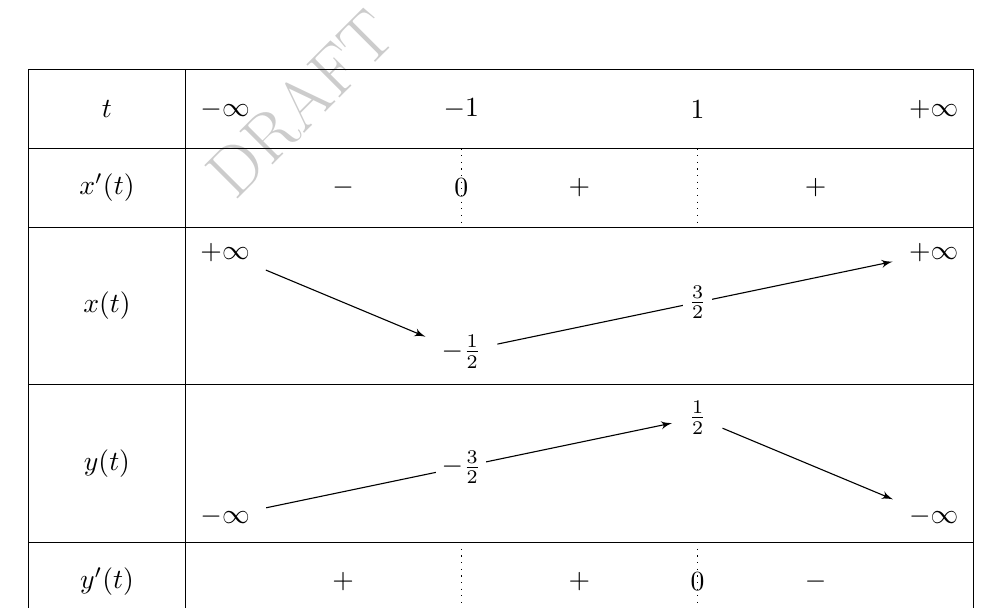
\begin{tikzpicture}
\tkzTabInit[lgt=2, espcl=3]{$t$ /1, $x'(t)$ /1, $x(t)$ /2, $y(t)$ /2, $y'(t)$ /1}{$-\infty$, $-1$, $1$, $+\infty$}
\tkzTabLine{ , -, z, +, t, +, }
\tkzTabVar{+/$+\infty$, -/$-\frac12$, R/, +/$+\infty$}
\tkzTabIma{2}{4}{3}{$\frac32$}
\tkzTabVar{-/$-\infty$, R/, +/$\frac12$, -/$-\infty$}
\tkzTabIma{1}{3}{2}{$-\frac32$}
\tkzTabLine{ , +, t, +, z, -, }
\end{tikzpicture}
\end{center}

\textbf{1.b) Tangentes parallèles aux axes.}

En un point de paramètre $t$, le vecteur $\vec V(t)=(x'(t),y'(t))=(1+t,1-t)$ ne s'annule jamais (on ne peut avoir à la fois $t=-1$ et $t=1$) : tous les points sont réguliers et $\vec V(t)$ dirige la tangente.
\begin{itemize}
\item Tangente parallèle à $(Oy)$ (verticale) : $x'(t)=0$, soit $t=-1$ : point $\big(-\frac12,-\frac32\big)$.
\item Tangente parallèle à $(Ox)$ (horizontale) : $y'(t)=0$, soit $t=1$ : point $\big(\frac32,\frac12\big)$.
\end{itemize}

\textbf{1.c) Intersections avec les axes et tangentes.}
\begin{itemize}
\item Avec $(Oy)$ : $x(t)=t\big(1+\frac t2\big)=0\iff t=0$ ou $t=-2$. Points $O(0,0)$ ($t=0$) et $A(0,-4)$ ($t=-2$).
\item Avec $(Ox)$ : $y(t)=t\big(1-\frac t2\big)=0\iff t=0$ ou $t=2$. Points $O(0,0)$ et $B(4,0)$ ($t=2$).
\end{itemize}
Vecteurs directeurs des tangentes : en $O$ ($t=0$) : $\vec V=(1,1)$ ; en $A$ ($t=-2$) : $\vec V=(-1,3)$ ; en $B$ ($t=2$) : $\vec V=(3,-1)$.

\textbf{1.d) Allure de la courbe.}
\begin{center}
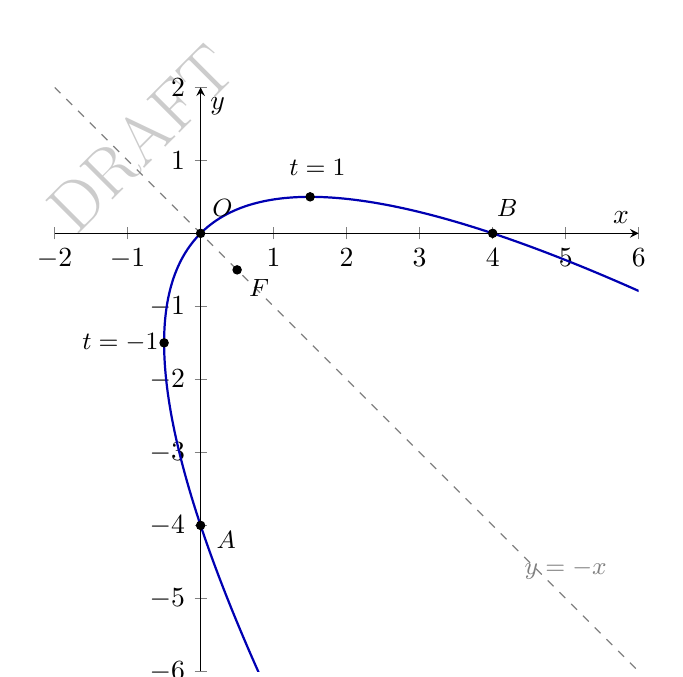
\begin{tikzpicture}
\begin{axis}[axis lines=middle, xlabel=$x$, ylabel=$y$, xmin=-2, xmax=6, ymin=-6, ymax=2, width=9cm, height=9cm, samples=200, domain=-3.6:3.6]
\addplot[blue!70!black, thick, variable=\t, parametric] ({t+t^2/2},{t-t^2/2});
\addplot[dashed, gray, domain=-2:6] {-x};
\addplot[only marks, mark=*, mark size=1.5pt] coordinates {(0,0) (0,-4) (4,0) (-0.5,-1.5) (1.5,0.5) (0.5,-0.5)};
\node at (axis cs:0.3,0.35) {\small $O$};
\node at (axis cs:0.35,-4.2) {\small $A$};
\node at (axis cs:4.2,0.35) {\small $B$};
\node at (axis cs:-1.1,-1.5) {\small $t=-1$};
\node at (axis cs:1.6,0.9) {\small $t=1$};
\node at (axis cs:0.8,-0.75) {\small $F$};
\node[gray] at (axis cs:5,-4.6) {\small $y=-x$};
\end{axis}
\end{tikzpicture}
\end{center}

\textbf{1.e) Équation cartésienne.} On a $x+y=2t$ et $x-y=t^2$. En éliminant $t=\frac{x+y}{2}$ :
\[
x-y=\frac{(x+y)^2}{4}\iff\boxed{v(x,y)=x^2+2xy+y^2-4x+4y=0}.
\]

\textbf{2.a) Nature de $h$.} $\dfrac{1+i}{\sqrt2}=\dfrac{\sqrt2}{2}+i\dfrac{\sqrt2}{2}=e^{i\pi/4}$, donc $Z=e^{i\pi/4}z$ : \textbf{$h$ est la rotation de centre $O$ et d'angle $\frac\pi4$}.

\textbf{2.b) Coordonnées de $M'$ et équation de $C'$.}
\[
Z=\frac{1}{\sqrt2}(1+i)(x+iy)=\frac{1}{\sqrt2}\big[(x-y)+i(x+y)\big],
\]
donc
\[
X(t)=\frac{x(t)-y(t)}{\sqrt2}=\frac{t^2}{\sqrt2},\qquad Y(t)=\frac{x(t)+y(t)}{\sqrt2}=\frac{2t}{\sqrt2}=\sqrt2\,t .
\]
En éliminant $t$ : $Y^2=2t^2=2\sqrt2\cdot\frac{t^2}{\sqrt2}=2\sqrt2\,X$. Une équation de $C'$ est
\[
\boxed{\varphi(X,Y)=Y^2-2\sqrt2\,X=0}.
\]
Réciproquement, tout point vérifiant cette équation est atteint ($t=\frac{Y}{\sqrt2}$).

$C'$ est une \textbf{parabole} de sommet $O$, d'axe $(OX)$, de la forme $Y^2=2pX$ avec $p=\sqrt2$ : son foyer est $F'\big(\frac{p}{2},0\big)=\big(\frac{\sqrt2}{2},0\big)$ et sa directrice la droite $X=-\frac{\sqrt2}{2}$.

\textbf{Nature de $C$.} $C'=h(C)$, donc $C=h^{-1}(C')$ où $h^{-1}$ est la rotation de centre $O$ et d'angle $-\frac\pi4$. Une rotation conserve les distances, donc transforme une parabole en parabole : \textbf{$C$ est une parabole} de sommet $O$, dont l'axe est l'image de $(OX)$ par la rotation d'angle $-\frac\pi4$, c'est-à-dire la \textbf{deuxième bissectrice} $y=-x$. Son foyer est $F=h^{-1}(F')$, d'affixe $\frac{\sqrt2}{2}e^{-i\pi/4}=\frac{1-i}{2}$, soit $F\big(\frac12,-\frac12\big)$, et sa directrice a pour équation $x-y+1=0$.

\medskip\textbf{Exercice 2}

Lois discrètes usuelles ($q=1-p$, $0<p<1$).

\begin{center}
\renewcommand{\arraystretch}{2.2}
\resizebox{\textwidth}{!}{%
\begin{tabular}{|l|c|c|c|c|}
\hline
\textbf{Loi} & \textbf{Valeurs} & $P(X=k)$ & $E(X)$ & $V(X)$\\
\hline
Uniforme sur $\{1,\dots,n\}$ & $1,\dots,n$ & $\dfrac1n$ & $\dfrac{n+1}{2}$ & $\dfrac{n^2-1}{12}$\\
\hline
Bernoulli $\mathcal{B}(p)$ & $0,1$ & $P(X=1)=p$, $P(X=0)=q$ & $p$ & $pq$\\
\hline
Binomiale $\mathcal{B}(n,p)$ & $0,\dots,n$ & $C_n^kp^kq^{n-k}$ & $np$ & $npq$\\
\hline
Poisson $\mathcal{P}(\lambda)$, $\lambda>0$ & $\mathbb{N}$ & $e^{-\lambda}\dfrac{\lambda^k}{k!}$ & $\lambda$ & $\lambda$\\
\hline
Géométrique $\mathcal{G}(p)$ & $\mathbb{N}^*$ & $pq^{k-1}$ & $\dfrac1p$ & $\dfrac{q}{p^2}$\\
\hline
Hypergéométrique $\mathcal{H}(N,n,p)$ & $\max(0,n-Nq)\le k\le\min(n,Np)$ & $\dfrac{C_{Np}^kC_{Nq}^{n-k}}{C_N^n}$ & $np$ & $npq\dfrac{N-n}{N-1}$\\
\hline
Pascal (rang du $r$-ième succès) & $r,r+1,\dots$ & $C_{k-1}^{r-1}p^rq^{k-r}$ & $\dfrac rp$ & $\dfrac{rq}{p^2}$\\
\hline
Binomiale négative (échecs avant le $r$-ième succès) & $\mathbb{N}$ & $C_{k+r-1}^{r-1}p^rq^{k}$ & $\dfrac{rq}{p}$ & $\dfrac{rq}{p^2}$\\
\hline
\end{tabular}}
\end{center}

\underline{Interprétations.}
\begin{itemize}
\item \emph{Bernoulli} : une épreuve à deux issues (succès de probabilité $p$).
\item \emph{Binomiale} : nombre de succès lors de $n$ épreuves de Bernoulli indépendantes de même paramètre $p$ (somme de $n$ variables de Bernoulli indépendantes, d'où $E=np$ et $V=npq$).
\item \emph{Poisson} : loi des évènements rares ; elle approche $\mathcal{B}(n,p)$ quand $n$ est grand, $p$ petit, avec $\lambda=np$.
\item \emph{Géométrique} : rang du premier succès dans une suite d'épreuves de Bernoulli indépendantes.
\item \emph{Hypergéométrique} : nombre d'éléments « marqués » dans un tirage simultané (sans remise) de $n$ éléments parmi $N$, dont une proportion $p$ est marquée.
\item \emph{Pascal} : rang du $r$-ième succès ; c'est la somme de $r$ variables géométriques indépendantes, d'où $E=\frac rp$ et $V=\frac{rq}{p^2}$.
\item \emph{Binomiale négative} : nombre d'échecs avant le $r$-ième succès ; si $X$ suit la loi de Pascal, $X-r$ suit la loi binomiale négative, d'où $E=\frac rp-r=\frac{rq}{p}$ et la même variance.
\end{itemize}

\medskip\textbf{Exercice 3}

Chaque mois, le versement augmente de $3\,\%$ : $U_{n+1}=U_n+0{,}03\,U_n=1{,}03\,U_n$, avec $U_1=600\,000$.

\textbf{1. Troisième mois.} $U_2=1{,}03\times600\,000=618\,000$ et
\[
U_3=1{,}03\times618\,000=\boxed{636\,540\ \text{FCFA}}.
\]

\textbf{2. Nature de $(U_n)$ et expression.} Comme $U_{n+1}=1{,}03\,U_n$ pour tout $n\ge1$, $(U_n)$ est une \textbf{suite géométrique de raison $q=1{,}03$ et de premier terme $U_1=600\,000$}. Donc, pour tout $n\ge1$ :
\[
\boxed{U_n=U_1\,q^{\,n-1}=600\,000\times1{,}03^{\,n-1}}.
\]
(Attention à l'exposant $n-1$ : le premier terme est $U_1$, pas $U_0$. On vérifie $U_1=600\,000$, $U_2=618\,000$.)

\textbf{3. Dernier mois ($n=12$).}
\[
U_{12}=600\,000\times1{,}03^{11}\approx600\,000\times1{,}384\,234\approx\boxed{830\,540\ \text{FCFA}}.
\]

\textbf{4. Somme totale.} $S$ est la somme des $12$ premiers termes d'une suite géométrique :
\[
S=U_1+U_2+\dots+U_{12}=U_1\big(1+q+\dots+q^{11}\big)=U_1\,\frac{q^{12}-1}{q-1}=600\,000\times\frac{1{,}03^{12}-1}{0{,}03}.
\]
Avec $1{,}03^{12}\approx1{,}425\,761$ : $\dfrac{1{,}03^{12}-1}{0{,}03}\approx14{,}192\,03$, d'où
\[
\boxed{S\approx8\,515\,218\ \text{FCFA}}.
\]
\remarque{Formule à retenir : la somme de $N$ termes consécutifs d'une suite géométrique de raison $q\neq1$ vaut $(\text{premier terme})\times\dfrac{1-q^{N}}{1-q}$, où $N$ est le \emph{nombre} de termes (ici $N=12$).}

\end{spacing}
\end{document}
